\section{Dữ liệu bảng: Phát hiện gian lận mở tài khoản ngân hàng}
\label{sec:tabular}

\subsection{Bối cảnh bài toán, toàn vẹn dữ liệu và phân chia theo thời gian}
Trong nghiệp vụ mở tài khoản ngân hàng trực tuyến, gian lận thường diễn ra dưới hình thức mạo danh hoặc tạo lập danh tính giả nhằm chiếm đoạt hạn mức tín dụng đi kèm. Hệ quả của sai số phân loại có tính bất đối xứng rõ rệt: bỏ sót hồ sơ gian lận gây tổn thất tài chính trực tiếp cho ngân hàng, trong khi chặn nhầm hồ sơ hợp pháp lại từ chối quyền tiếp cận dịch vụ tài chính cơ bản của khách hàng. Thực nghiệm trong chương này sử dụng tập dữ liệu chuẩn \texttt{Base.csv} thuộc bộ \textit{Bank Account Fraud (BAF)} \cite{jesus2022turning}, được tổng hợp bằng CTGAN từ dữ liệu ngân hàng thực đã ẩn danh, gồm \textbf{1.000.000 hồ sơ} trải dài qua 8 tháng (mã hóa \texttt{month} từ 0 đến 7) với \textbf{32 thuộc tính} (18 cột nguyên, 9 cột thực, 5 cột phân loại) và không có bản ghi trùng lặp hoàn toàn.

Kiểm tra bước đầu cho thấy ba đặc điểm cần xử lý trước khi phân tích sâu. Thứ nhất, biến mục tiêu \texttt{fraud\_bool} mất cân bằng nặng (\Cref{fig:tab_dist_shift}, bên trái): chỉ có 11.029 hồ sơ gian lận (1,10\%) so với 988.971 hồ sơ hợp pháp (98,90\%), tức xấp xỉ 1 ca gian lận trên 89 hồ sơ. Với tỷ lệ này, thước đo \textit{Accuracy} trở nên vô nghĩa vì một bộ phân loại luôn dự đoán hợp pháp đã đạt 98,90\% nhưng bỏ lọt toàn bộ gian lận. Do đó, thước đo chính được áp dụng theo \cite{jesus2022turning} là \textbf{TPR@5\%FPR} (tỷ lệ phát hiện gian lận khi khống chế tỷ lệ báo động nhầm đối với khách hàng hợp pháp không vượt quá 5\%), đi kèm \textit{ROC-AUC}, \textit{PR-AUC} và ma trận nhầm lẫn.

Thứ hai, dù Pandas ghi nhận 0 giá trị \texttt{NaN} mặc định, đối chiếu với tài liệu đặc tả dữ liệu cho thấy cột \texttt{device\_fraud\_count} chỉ mang một giá trị hằng số duy nhất là \texttt{0} nên được loại bỏ, đồng thời 6 cột thực chất mã hóa dữ liệu khuyết bằng số âm: giá trị \texttt{-1} ở \texttt{prev\_address\_months\_count} (712.920 dòng), \texttt{bank\_months\_count} (253.635 dòng), \texttt{current\_address\_months\_count} (4.254 dòng), \texttt{session\_length\_in\_minutes} (2.015 dòng), \texttt{device\_distinct\_emails\_8w} (359 dòng) và mọi giá trị âm ($< 0$) ở \texttt{intended\_balcon\_amount} (742.523 dòng, chiếm 74,25\%). Riêng 488 dòng mang giá trị \texttt{-1} ở \texttt{credit\_risk\_score} nằm trong miền điểm hợp lệ $[-191, 389]$ nên được giữ nguyên. Với 6 cột khuyết ẩn này, giá trị khuyết được chuẩn hóa về \texttt{NaN} sau khi tạo tương ứng 6 cột cờ nhị phân \texttt{\_flag} nhằm bảo lưu tín hiệu hành vi không khai báo thông tin.

Thứ ba, tỷ lệ gian lận không dừng theo thời gian (\Cref{fig:tab_dist_shift}, bên phải): dao động trong khoảng 0,875\%--1,183\% từ tháng 0 đến tháng 5, rồi tăng lên 1,341\% ở tháng 6 và 1,475\% ở tháng 7, trong khi lượng hồ sơ giảm dần từ 150.936 (tháng 3) xuống 96.843 (tháng 7). Sự hiện diện của \textit{temporal shift} khiến phép chia ngẫu nhiên (trộn lẫn các tháng) tạo ra rò rỉ thông tin tương lai (\textit{look-ahead bias}). Vì vậy, dữ liệu được tách nghiêm ngặt theo trục thời gian (\textit{Temporal Split}, \Cref{tab:tab_split}); mọi khảo sát EDA, tính toán thống kê và khớp bộ tiền xử lý từ đây trở đi chỉ tiến hành trên tập Train.

\begin{figure}[H]
  \centering
  \begin{minipage}[b]{0.47\linewidth}
    \centering
    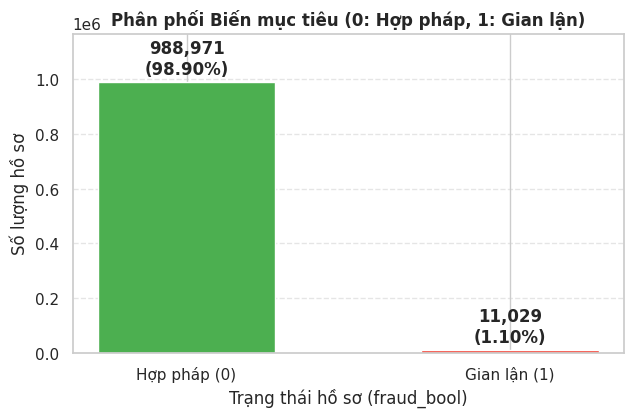
\includegraphics[width=\linewidth]{tabular/c13_f0.png}
  \end{minipage}\hfill
  \begin{minipage}[b]{0.51\linewidth}
    \centering
    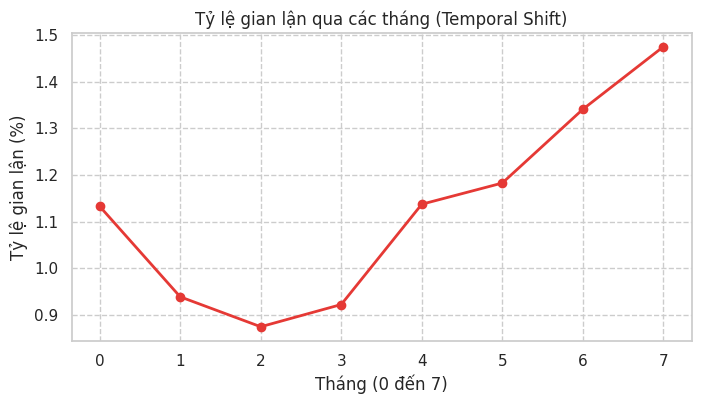
\includegraphics[width=\linewidth]{tabular/c25_f0.png}
  \end{minipage}
  \caption{Phân phối biến mục tiêu \texttt{fraud\_bool} (trái) và biến động tỷ lệ gian lận qua 8 tháng (phải) trên toàn tập \texttt{Base.csv}.}
  \label{fig:tab_dist_shift}
\end{figure}

\begin{table}[H]
  \centering
  \caption{Cấu trúc phân chia theo thời gian (\textit{Temporal Split}) của tập \texttt{Base.csv}.}
  \label{tab:tab_split}
  \resizebox{\linewidth}{!}{%
  \begin{tabular}{l c r r c c}
    \toprule
    \textbf{Tập dữ liệu} & \textbf{Tháng} & \textbf{Số hồ sơ} & \textbf{Số ca gian lận} & \textbf{Tỷ trọng (\%)} & \textbf{Tỷ lệ gian lận (\%)} \\
    \midrule
    Train & 0 -- 5 & 794.989 & 8.151 & 79,50 & 1,03 \\
    Validation & 6 & 108.168 & 1.450 & 10,82 & 1,34 \\
    Test & 7 & 96.843 & 1.428 & 9,68 & 1,47 \\
    \bottomrule
  \end{tabular}%
  }
\end{table}

\subsection{Khám phá dữ liệu trên tập huấn luyện}

\subsubsection{Cơ chế dữ liệu khuyết và ảnh hưởng của việc điền trung vị}
Để kiểm tra việc bỏ trống thông tin là ngẫu nhiên (\textit{MCAR}) hay gắn với hành vi rủi ro (\textit{MNAR}), tỷ lệ gian lận được đối chiếu giữa nhóm thiếu (\texttt{flag = 1}) và nhóm khai báo đủ (\texttt{flag = 0}) thông qua tỷ số rủi ro (\textit{Risk Ratio}) trên \texttt{df\_train}. Kết quả ở \Cref{fig:tab_missing} cho thấy dữ liệu khuyết mang tín hiệu phân tách mạnh ở ba cột thiếu nhiều nhất: với \texttt{prev\_address\_months\_count} (thiếu 71,50\%), nhóm không khai báo có tỷ lệ gian lận 1,32\% so với chỉ 0,28\% ở nhóm có khai báo địa chỉ cũ (chênh lệch \textbf{4,73 lần}); tương tự, rủi ro tăng \textbf{2,58 lần} khi thiếu \texttt{intended\_balcon\_amount} (1,22\% vs 0,47\%) và \textbf{1,80 lần} khi thiếu \texttt{bank\_months\_count} (1,54\% vs 0,85\%). Ba cột còn lại thiếu dưới 0,4\% và có tỷ số rủi ro gần trung tính.

\begin{figure}[H]
  \centering
  \begin{minipage}[b]{0.55\linewidth}
    \centering
    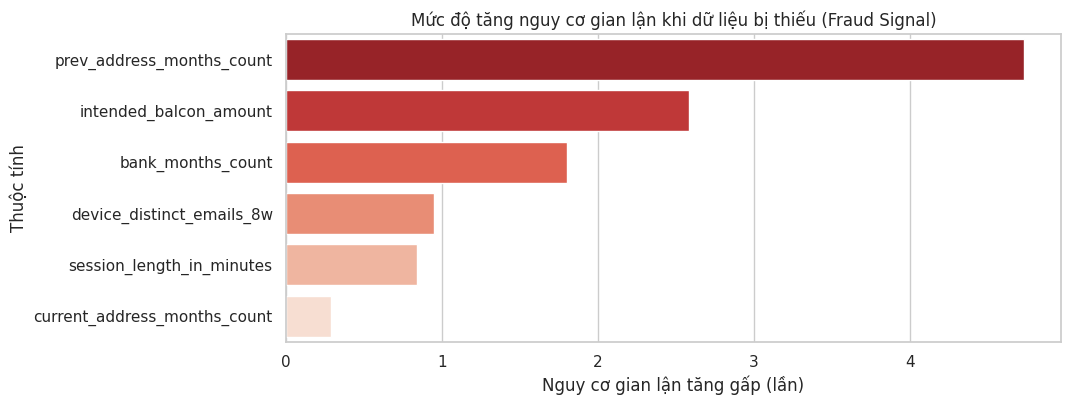
\includegraphics[width=\linewidth]{tabular/c31_f0.png}
  \end{minipage}\hfill
  \begin{minipage}[b]{0.43\linewidth}
    \centering
    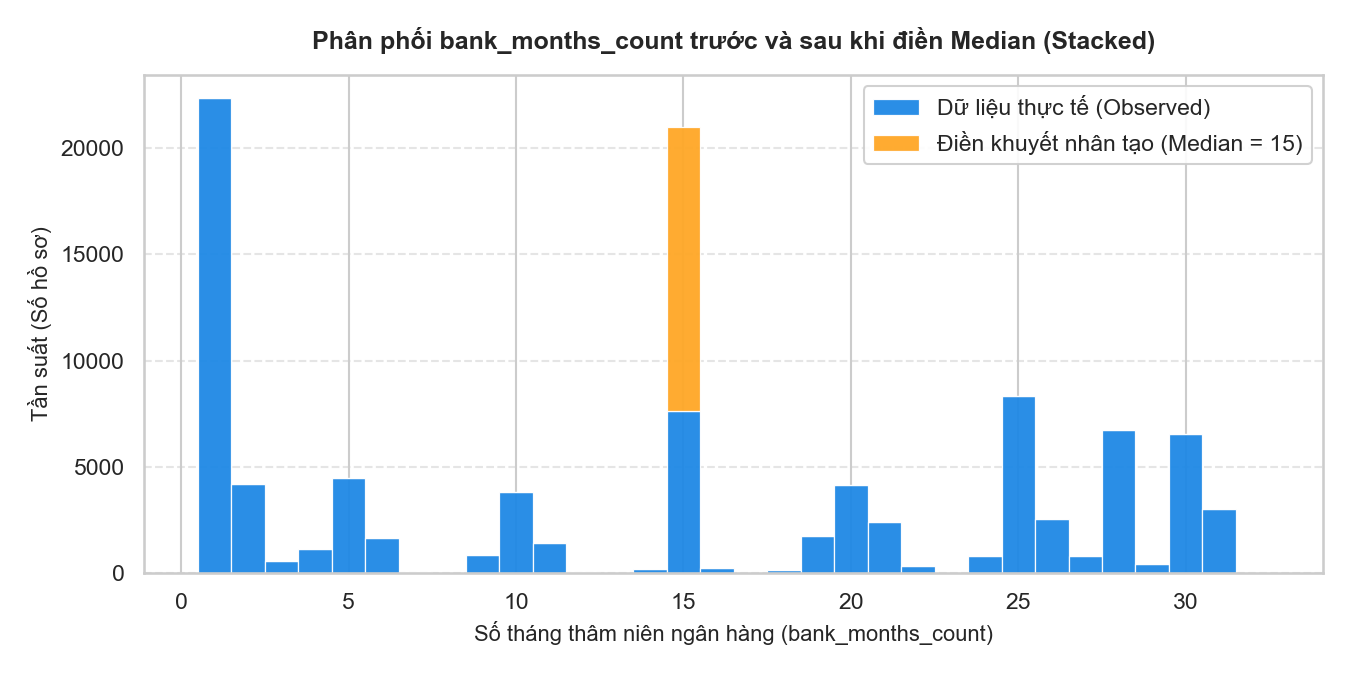
\includegraphics[width=\linewidth]{tabular/c33_f0.png}
  \end{minipage}
  \caption{Tỷ số tăng nguy cơ gian lận khi khuyết dữ liệu (trái) và biến dạng phân phối của \texttt{bank\_months\_count} khi điền trung vị bằng 15 tháng (phải).}
  \label{fig:tab_missing}
\end{figure}

Thử nghiệm điền khuyết bằng trung vị (\textit{median} = 15,0 tháng) trên \texttt{bank\_months\_count} (\Cref{fig:tab_missing}, bên phải) tạo ra một đỉnh nhọn nhân tạo chiếm 25,10\% mẫu, làm méo phân phối thực và trộn lẫn nhóm bỏ trống với nhóm có thâm niên tài khoản 15 tháng. Do đó, tập dữ liệu được giữ nguyên giá trị \texttt{NaN} kết hợp 6 cờ \texttt{\_flag} cho mô hình cây; phép điền trung vị chỉ áp dụng nội bộ trong pipeline của mô hình tuyến tính.

\subsubsection{Phân hóa rủi ro theo biến phân loại, kênh nộp đơn và hành vi phiên}
Khảo sát nhóm biến phân loại và cờ định danh trên \texttt{df\_train} (\Cref{fig:tab_cat_flags}) ghi nhận sự phân hóa rõ rệt quanh mức nền 1,03\%. Ở biến hệ điều hành (\texttt{device\_os}), nhóm \texttt{windows} (26,8\% hồ sơ) có tỷ lệ gian lận 2,30\%, cao hơn gấp đôi mức nền, theo sau là \texttt{macintosh} (1,26\%), trong khi \texttt{linux} và \texttt{other} ở quanh mức 0,5\%. Với phương thức thanh toán (\texttt{payment\_type}), nhóm \texttt{AC} dẫn đầu ở mức 1,58\%, còn ở tình trạng nhà ở (\texttt{housing\_status}), nhóm \texttt{BA} ghi nhận tỷ lệ rủi ro nổi bật nhất so với các nhóm còn lại.

\begin{figure}[H]
  \centering
  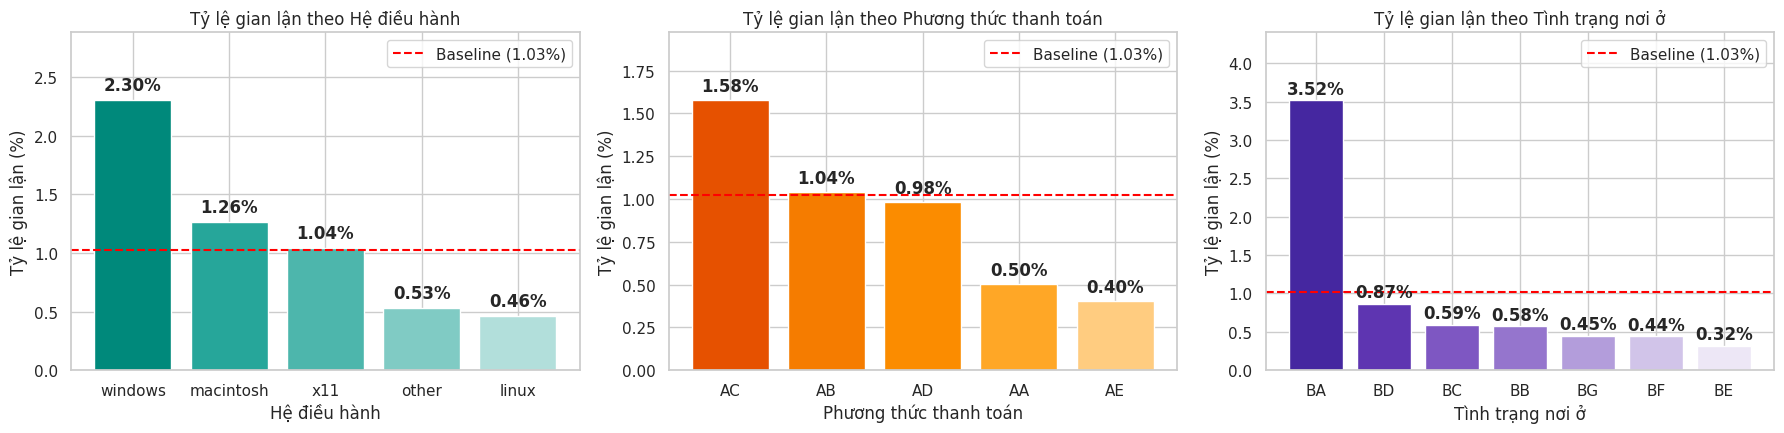
\includegraphics[width=0.96\linewidth]{tabular/c36_f0.png}\\[4pt]
  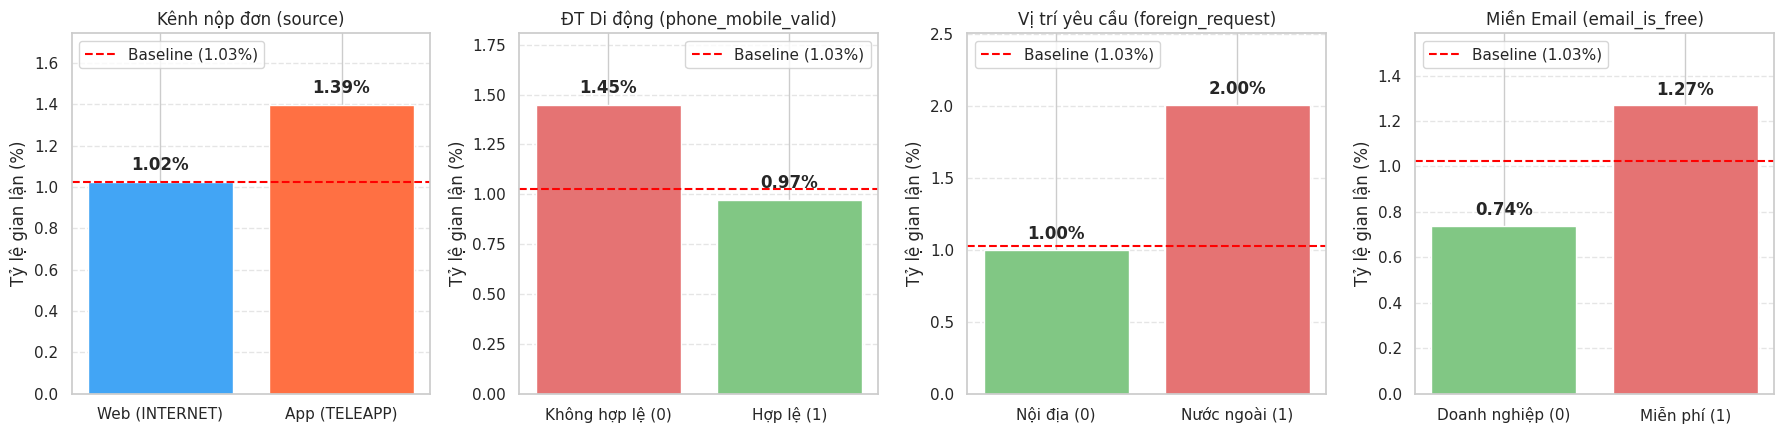
\includegraphics[width=0.96\linewidth]{tabular/c38_f0.png}\\[4pt]
  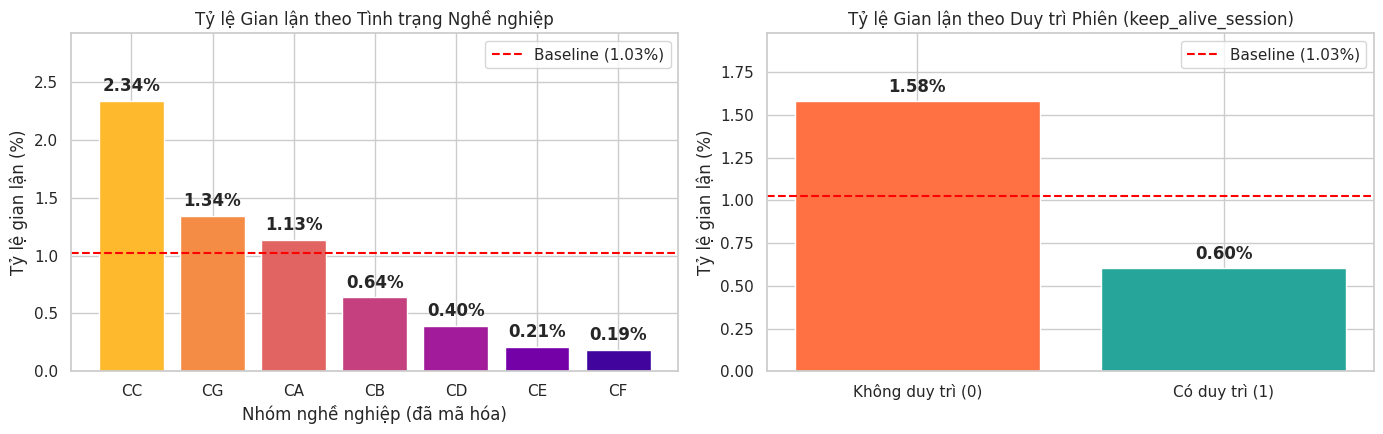
\includegraphics[width=0.80\linewidth]{tabular/c40_f0.png}
  \caption{Tỷ lệ gian lận trên tập huấn luyện phân theo các biến phân loại chính (trên), nhóm cờ định danh -- kênh nộp đơn (giữa), tình trạng nghề nghiệp và duy trì phiên (dưới).}
  \label{fig:tab_cat_flags}
\end{figure}

Xét các cờ xác thực và hành vi phiên, yêu cầu xuất phát từ nước ngoài (\texttt{foreign\_request = 1}) có tỷ lệ gian lận 2,00\% so với 1,00\% nội địa; hồ sơ không duy trì phiên (\texttt{keep\_alive\_session = 0}) có rủi ro 1,58\% so với 0,60\% khi duy trì; số điện thoại di động hoặc cố định không hợp lệ (\texttt{phone\_mobile\_valid = 0}: 1,45\%; \texttt{phone\_home\_valid = 0}: 1,29\%) và email miễn phí (\texttt{email\_is\_free = 1}: 1,27\% vs 0,74\%) đều gắn với mức rủi ro cao hơn. Kênh ứng dụng di động (\texttt{TELEAPP}) tuy chỉ chiếm 5.737 đơn nhưng có tỷ lệ gian lận 1,39\% so với 1,02\% của kênh web (\texttt{INTERNET}). Đáng chú ý, tình trạng nghề nghiệp (\texttt{employment\_status}) phân hóa tới hơn 12 lần, từ 2,34\% ở nhóm \texttt{CC} xuống còn 0,19\% ở nhóm \texttt{CF}.

\subsubsection{Biến vận tốc, giá trị ngoại lai và tín hiệu thiết bị}
Một giả thuyết phổ biến trong phòng chống gian lận là tốc độ nộp đơn quá cao (\texttt{velocity\_6h}) thường phản ánh tấn công tự động. Tuy nhiên, kiểm tra bằng quy tắc IQR (ngưỡng trên 14.326,7 đơn/giờ, chiếm 6.498 hồ sơ hay 0,82\%) và phân tầng theo thập phân vị (\Cref{fig:tab_velocity}) lại cho kết quả ngược chiều: nhóm ngoại lai chỉ có tỷ lệ gian lận 0,65\% (thấp hơn mức nền 1,03\%), và tỷ lệ gian lận giảm gần như đơn điệu từ 1,34\% ở thập phân vị thấp nhất (D1) xuống 0,70\% ở thập phân vị cao nhất (D10). Do ngoại lai không phải là nhiễu đo lường hay cụm gian lận riêng biệt, toàn bộ các điểm cực trị (kể cả 20 hồ sơ có \texttt{velocity\_6h < 0}) đều được giữ lại thay vì cắt bỏ.

\begin{figure}[H]
  \centering
  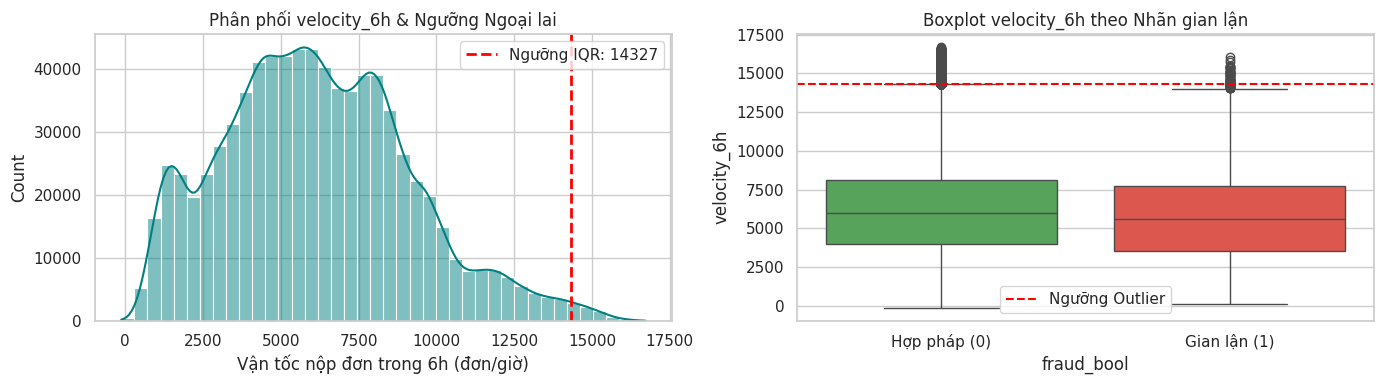
\includegraphics[width=0.92\linewidth]{tabular/c42_f0.png}\\[4pt]
  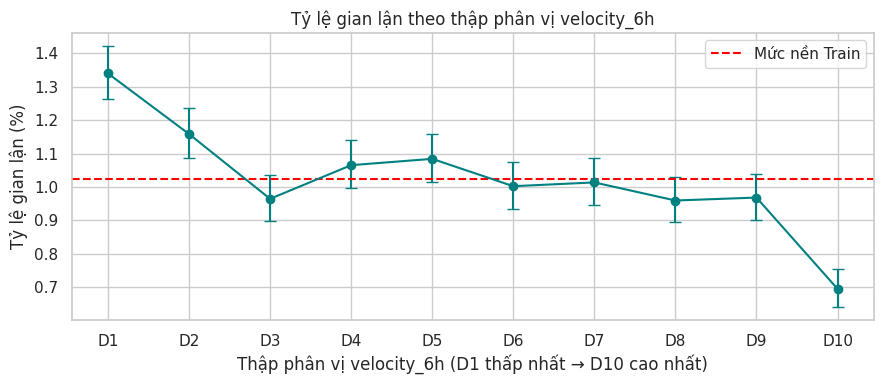
\includegraphics[width=0.68\linewidth]{tabular/c42_f1.png}
  \caption{Phân phối, ngưỡng ngoại lai IQR của \texttt{velocity\_6h} (trên) và tỷ lệ gian lận giảm dần theo 10 thập phân vị vận tốc (dưới).}
  \label{fig:tab_velocity}
\end{figure}

Ba khung vận tốc (\texttt{velocity\_6h}, \texttt{velocity\_24h}, \texttt{velocity\_4w}) chỉ có tương quan tuyến tính ở mức trung bình ($r \in [0,30; 0,40]$), bổ trợ thông tin cho nhau mà không gây đa cộng tuyến nghiêm trọng. Với các biến hành vi và thiết bị khác (\Cref{fig:tab_behavior}), độ trễ nộp đơn \texttt{days\_since\_request} từ 1 đến 5 ngày ghi nhận rủi ro 1,99\% (gấp đôi nhóm nộp ngay trong ngày là 1,01\%); hồ sơ phát sinh tại chi nhánh không có lưu lượng trong 8 tuần (\texttt{bank\_branch\_count\_8w = 0}) đạt 1,68\% so với 0,72\% ở chi nhánh có trên 100 đơn; và phiên thao tác kéo dài trên 30 phút đạt 1,80\% so với mức 0,98\%--1,05\% của phiên 2--15 phút. Đặc biệt, khi một thiết bị được sử dụng với 2 địa chỉ email khác nhau trong 8 tuần (\texttt{device\_distinct\_emails\_8w = 2}, 22.583 đơn), tỷ lệ gian lận tăng lên \textbf{3,88\%}, gấp gần 4 lần mức nền; ngược lại, \texttt{date\_of\_birth\_distinct\_emails\_4w} có xu hướng giảm rủi ro khi số email tăng (từ 1,81\% ở nhóm $\le 5$ về 0,61\%, $r = -0,043$).

\begin{figure}[H]
  \centering
  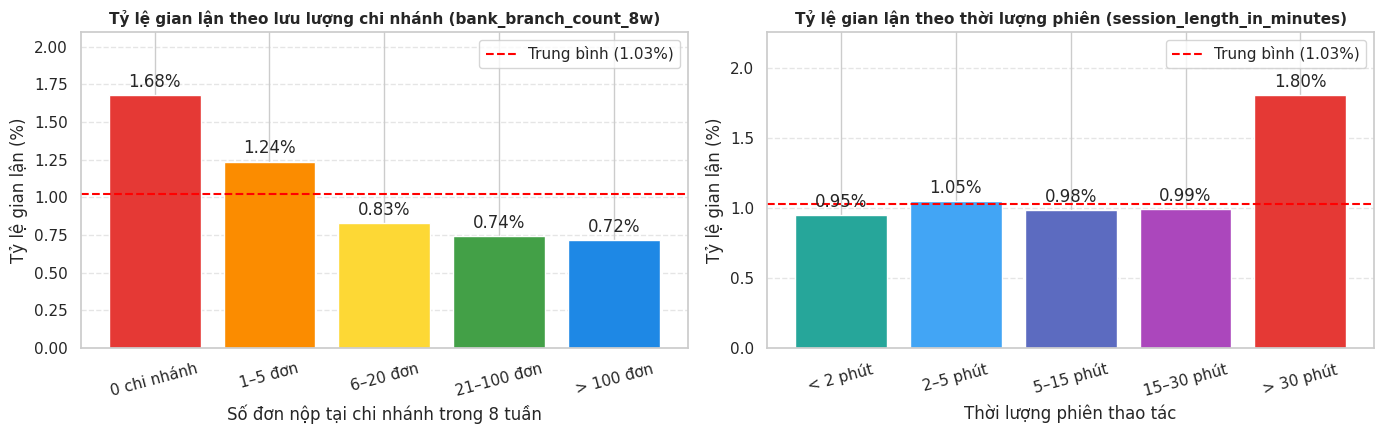
\includegraphics[width=0.88\linewidth]{tabular/c46_f0.png}\\[4pt]
  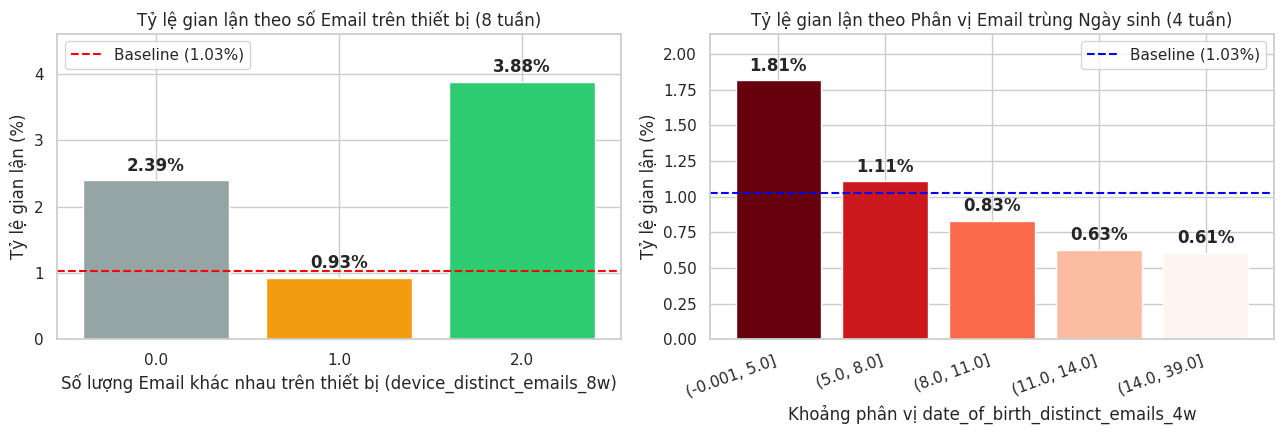
\includegraphics[width=0.88\linewidth]{tabular/c48_f0.png}
  \caption{Tỷ lệ gian lận theo lưu lượng chi nhánh, thời lượng phiên (trên) và theo số email dùng chung thiết bị, ngày sinh (dưới).}
  \label{fig:tab_behavior}
\end{figure}

\subsubsection{Đặc trưng tài chính, tương tác phi tuyến và độ ổn định phân phối}
Ở nhóm biến tài chính, hạn mức tín dụng do ứng viên tự đề xuất (\texttt{proposed\_credit\_limit}) tỷ lệ thuận với rủi ro: tăng từ 0,68\% (mức $\le 200$) lên 0,96\% (201--500) và 1,90\% ($> 500$). Ngược lại, việc đã sở hữu thẻ khác tại cùng ngân hàng (\texttt{has\_other\_cards = 1}) đóng vai trò tín hiệu an toàn rõ rệt (0,41\% so với 1,20\%).

Quan trọng hơn, phân tích hai chiều phát hiện các cụm tương tác phi tuyến mạnh (\Cref{fig:tab_interactions}). Khi kết hợp \texttt{credit\_risk\_score > 300} với hạn mức đề xuất cao $(1500, 2100]$, tỷ lệ gian lận vọt lên \textbf{19,62\%} (82/418 hồ sơ, CI 95\% Wilson $[16,09\%; 23,69\%]$), gấp khoảng 19 lần mức nền (kiểm chứng trên Validation tháng 6 vẫn giữ mức 16,05\%, tương quan hạng Spearman giữa hai tập đạt $\rho = 0,712$). Tương tự, tổ hợp \texttt{housing\_status = BA} và \texttt{device\_os = windows} đạt tỷ lệ gian lận \textbf{6,31\%} trên 45.597 hồ sơ (CI 95\% $[6,09\%; 6,54\%]$), trong khi tổ hợp \texttt{BE $\times$ linux} chỉ là 0,17\%.

\begin{figure}[H]
  \centering
  \begin{minipage}[b]{0.49\linewidth}
    \centering
    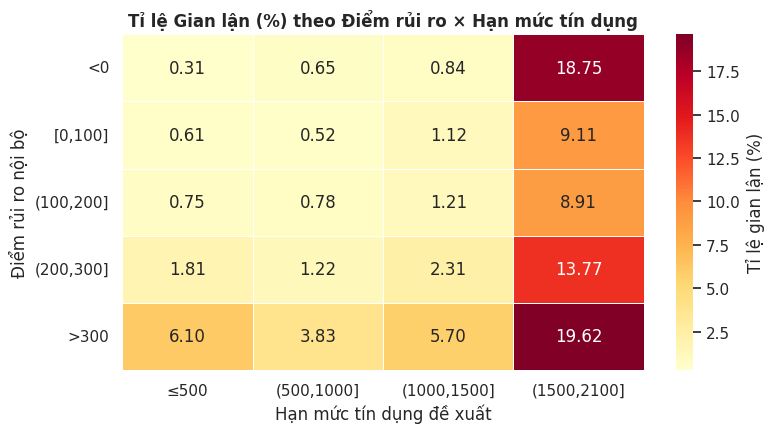
\includegraphics[width=\linewidth]{tabular/c52_f0.png}
  \end{minipage}\hfill
  \begin{minipage}[b]{0.49\linewidth}
    \centering
    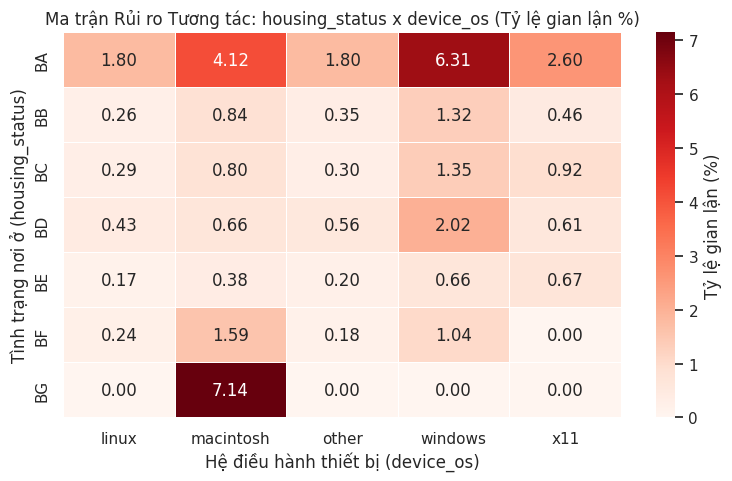
\includegraphics[width=\linewidth]{tabular/c56_f0.png}
  \end{minipage}
  \caption{Bản đồ nhiệt tương tác phi tuyến: điểm rủi ro tín dụng $\times$ hạn mức đề xuất (trái) và tình trạng nhà ở $\times$ hệ điều hành thiết bị (phải).}
  \label{fig:tab_interactions}
\end{figure}

Đánh giá toàn diện 31 thuộc tính còn lại bằng Thông tin tương hỗ (\textit{Mutual Information -- MI}) cho thấy các biến phân loại và cờ hành vi dẫn đầu về khả năng phân tách phi tuyến (\texttt{housing\_status}: 0,0367; \texttt{prev\_address\_months\_count}: 0,0288; \texttt{device\_os}: 0,0258; \texttt{keep\_alive\_session}: 0,0244; \texttt{intended\_balcon\_amount}: 0,0233). Kiểm tra chỉ số ổn định phân phối (\textit{Population Stability Index -- PSI}) giữa nửa đầu (tháng 0--2) và nửa sau (tháng 3--5) của tập Train cho thấy phần lớn biến ổn định ($\text{PSI} < 0,10$), ngoại trừ nhóm vận tốc biến động mạnh theo mùa vụ (\texttt{velocity\_4w}: 4,1643; \texttt{velocity\_24h}: 0,6191; \texttt{velocity\_6h}: 0,2925) và \texttt{credit\_risk\_score} (0,2744).

\subsubsection{Chênh lệch nhân khẩu học và tiền đề đánh giá công bằng}
Khảo sát các thuộc tính nhạy cảm (\Cref{fig:tab_demo}) cho thấy tỷ lệ gian lận tăng đều theo độ tuổi: từ 0,33\% ở nhóm 10 tuổi và 0,45\% ở nhóm 20 tuổi lên 1,12\% ở tuổi 40 và 3,08\% ở tuổi 60 (theo \cite{jesus2022turning}, kẻ gian thường nhắm mạo danh người lớn tuổi do nhóm này có uy tín tín dụng cao hơn). Khi tách theo ngưỡng 50 tuổi, nhóm $\ge 50$ tuổi chỉ chiếm 18,77\% hồ sơ (149.234 đơn) nhưng có tỷ lệ gian lận 2,21\%, gấp \textbf{2,94 lần} nhóm $< 50$ tuổi (0,75\% trên 645.755 đơn). Tương tự, tỷ số chênh lệch (\textit{Disparity Ratio}) giữa nhóm thu nhập cao ($> 0,6$: 1,33\%) và thu nhập thấp ($\le 0,3$: 0,58\%) là 2,28 lần, còn giữa nhóm nghề nghiệp \texttt{CC} và \texttt{CF} là 12,45 lần. Sự khác biệt về tỷ lệ nền (\textit{prevalence}) này báo trước nguy cơ một mô hình dùng ngưỡng phân loại chung sẽ gây tỷ lệ báo động nhầm cao hơn nhiều cho nhóm khách hàng lớn tuổi.

\begin{figure}[H]
  \centering
  \begin{minipage}[b]{0.47\linewidth}
    \centering
    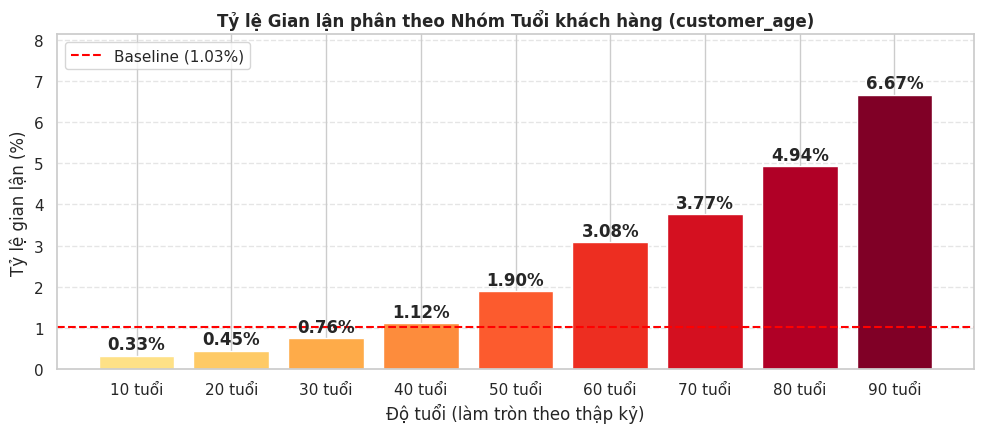
\includegraphics[width=\linewidth]{tabular/c62_f0.png}
  \end{minipage}\hfill
  \begin{minipage}[b]{0.51\linewidth}
    \centering
    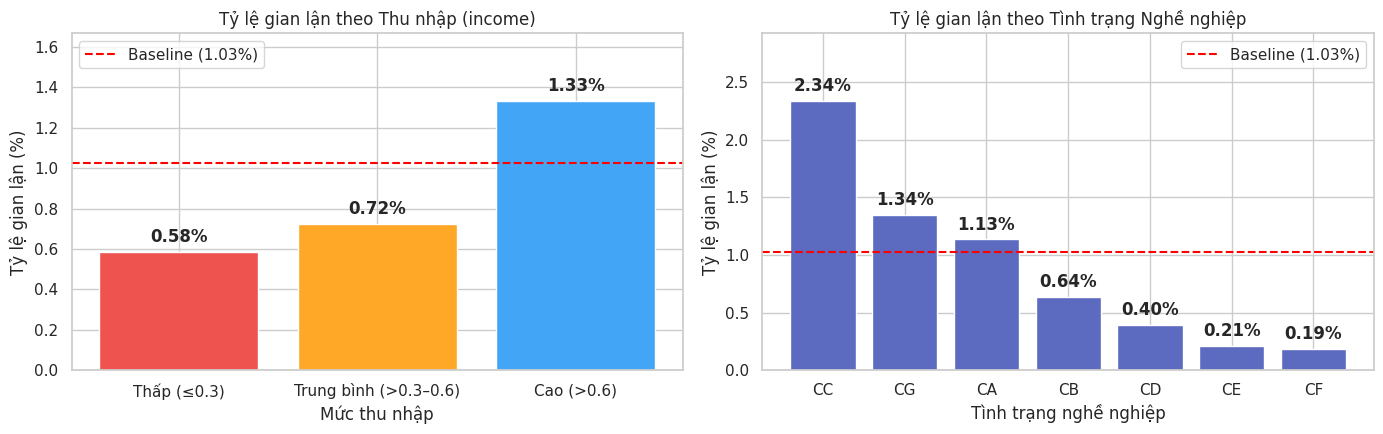
\includegraphics[width=\linewidth]{tabular/c66_f0.png}
  \end{minipage}
  \caption{Tỷ lệ gian lận tăng dần theo độ tuổi (trái) và chênh lệch rủi ro nền theo mức thu nhập, tình trạng nghề nghiệp (phải) trên \texttt{df\_train}.}
  \label{fig:tab_demo}
\end{figure}

\subsection{Tiền xử lý, kỹ thuật đặc trưng và thiết lập mô hình}
Nhằm giúp mô hình cây nắm bắt các quan hệ tỷ lệ và giảm tác động của trôi dạt vận tốc theo mùa vụ, nhóm bổ sung \textbf{6 đặc trưng tỷ lệ} gồm: hai tỷ lệ vận tốc ngắn/dài hạn (\texttt{vel\_6h\_24h}, \texttt{vel\_24h\_4w}), thâm niên cư trú và ngân hàng chuẩn hóa theo tuổi (\texttt{addr\_per\_age}, \texttt{bank\_per\_age}), và hai tỷ lệ hạn mức, tiền nạp so với thu nhập (\texttt{limit\_per\_income}, \texttt{balcon\_per\_income}). Tổng cộng đầu vào gồm \textbf{42 đặc trưng} (36 biến số bao gồm 6 cờ \texttt{\_flag} và 6 tỷ lệ mới, 5 biến phân loại, cùng biến \texttt{month}). Thử nghiệm \textit{ablation} với 3 seed trên biến \texttt{month} cho thấy việc loại bỏ \texttt{month} làm \texttt{TPR@5\%FPR} thay đổi $+0,010$ (CI 95\% $[-0,015; +0,022]$, không có ý nghĩa thống kê); do đó \texttt{month} được giữ lại như lựa chọn nhất quán giữa các bảng thực nghiệm, đi kèm lưu ý biến này không thể ngoại suy vượt ngoài miền tháng 0--5.

Để chọn phương pháp chuẩn hóa cho mô hình tuyến tính, \Cref{fig:tab_scaling} đối chiếu phân phối gốc với \texttt{StandardScaler} và \texttt{RobustScaler} trên \texttt{velocity\_6h} và \texttt{intended\_balcon\_amount}. Nhờ dựa trên trung vị và khoảng tứ phân vị (IQR), \texttt{RobustScaler} giữ nguyên cấu trúc phân phối và hạn chế hiện tượng co cụm dữ liệu bình thường do ảnh hưởng của ngoại lai.

\begin{figure}[H]
  \centering
  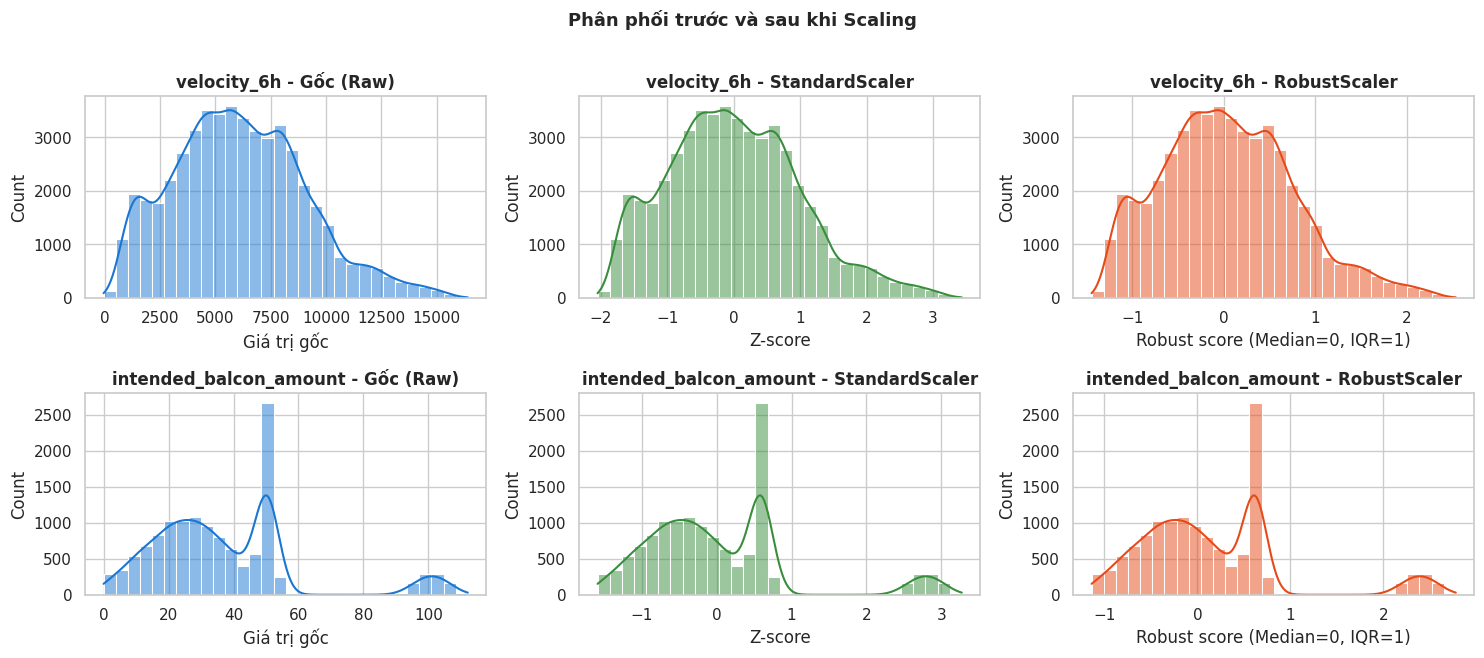
\includegraphics[width=0.90\linewidth]{tabular/c68_f0.png}
  \caption{Phân phối của \texttt{velocity\_6h} và \texttt{intended\_balcon\_amount} trước và sau chuẩn hóa bằng \texttt{StandardScaler} và \texttt{RobustScaler} trên \texttt{df\_train}.}
  \label{fig:tab_scaling}
\end{figure}

Hai họ mô hình được huấn luyện theo quy trình tách biệt hoàn toàn trên \texttt{df\_train}:
\begin{itemize}[leftmargin=*]
  \item \textbf{Logistic Regression (mô hình cơ sở):} sử dụng \texttt{SimpleImputer(median)}, \texttt{RobustScaler} và \texttt{OneHotEncoder} đóng gói trong \texttt{Pipeline}, kèm tham số \texttt{class\_weight='balanced'} để bù mất cân bằng lớp.
  \item \textbf{LightGBM (mô hình chính):} giữ nguyên giá trị \texttt{NaN}, xử lý trực tiếp biến phân loại dạng \texttt{category}, sử dụng siêu tham số tham khảo từ \cite{jesus2022turning} với dừng sớm (\textit{early stopping}) theo Validation AUC và lấy trung bình dự đoán từ 3 seed độc lập (số cây tối ưu lần lượt là 438, 637 và 531 cây) nhằm giảm phương sai ước lượng.
\end{itemize}

Ngưỡng phân loại được chọn duy nhất trên Validation (tháng 6) tại điểm $\text{FPR} \le 5\%$ — thu được ngưỡng \textbf{0,7781} cho Logistic Regression và \textbf{0,0478} cho LightGBM — sau đó khóa cứng để đánh giá một lần trên Test (tháng 7).

\subsection{Kết quả thực nghiệm, giải thích mô hình và kiểm chứng giả thuyết}

\subsubsection{Hiệu năng phân loại, đối chiếu tài liệu gốc và kiểm định Bootstrap}
\Cref{tab:tab_results} tổng hợp kết quả của hai mô hình trên Validation và Test, đặt cạnh mốc tham chiếu của bài báo gốc NeurIPS 2022 \cite{jesus2022turning}. Trên tập Test (96.843 hồ sơ, 1.428 ca gian lận), LightGBM đạt \texttt{TPR@FPR5\%} xếp hạng bằng \textbf{0,5798}, tái lập sát và nhỉnh hơn mốc 0,5600 công bố trong bài báo gốc. Khi khóa ngưỡng từ tháng 6 sang tháng 7 (\texttt{TPR@ngưỡng}), LightGBM phát hiện được 793 ca gian lận (55,53\%, giảm 19,0\% số ca bỏ lọt so với 644 ca của Logistic Regression) với FPR thực tế ở mức 4,22\%, vẫn nằm trong ngân sách 5\%. Khoảng cách giữa \texttt{TPR@FPR5\%} (0,580) và \texttt{TPR@ngưỡng} (0,555) phản ánh hiện tượng ngưỡng cố định trở nên chặt hơn khi tỷ lệ gian lận tháng 7 tăng cao, gợi ý cần hiệu chỉnh lại ngưỡng định kỳ theo phân vị lưu lượng cảnh báo khi vận hành.

\begin{table}[H]
  \centering
  \caption{Hiệu năng Logistic Regression và LightGBM trên Validation (tháng 6), Test (tháng 7) và đối chiếu với mốc bài báo gốc \cite{jesus2022turning}.}
  \label{tab:tab_results}
  \resizebox{\linewidth}{!}{%
  \begin{tabular}{l l c c c c c c}
    \toprule
    \textbf{Tập / Nguồn} & \textbf{Mô hình} & \textbf{TPR@FPR5\%} & \textbf{TPR@ngưỡng} & \textbf{FPR} & \textbf{Precision} & \textbf{ROC-AUC} & \textbf{PR-AUC} \\
    \midrule
    Val (Tháng 6) & Logistic Regression & 0,5069 & 0,5069 & 0,0495 & 0,1221 & 0,8829 & 0,1565 \\
    Val (Tháng 6) & LightGBM & 0,5310 & 0,5310 & 0,0496 & 0,1270 & 0,8948 & 0,1822 \\
    \midrule
    Test (Tháng 7) & Logistic Regression & 0,5301 & 0,4510 & 0,0348 & 0,1624 & 0,8868 & 0,1849 \\
    Test (Tháng 7) & LightGBM & \textbf{0,5798} & \textbf{0,5553} & 0,0422 & \textbf{0,1647} & \textbf{0,8986} & \textbf{0,2173} \\
    \midrule
    Paper \cite{jesus2022turning} & Logistic Regression & $\sim 0,5100$ & -- & 0,0500 & -- & -- & -- \\
    Paper \cite{jesus2022turning} & LightGBM & 0,5600 & -- & 0,0500 & -- & -- & -- \\
    \bottomrule
  \end{tabular}%
  }
\end{table}

Do tập Test chỉ chứa 1.428 ca gian lận, sai số lấy mẫu có thể lên tới $\pm 0,025$ điểm TPR. Kết quả lấy mẫu cặp \textit{Bootstrap} phân tầng 1.000 lần (\Cref{tab:tab_bootstrap}) cho thấy khoảng tin cậy 95\% của chênh lệch giữa LightGBM và Logistic Regression hoàn toàn nằm trên 0 ở cả ba chỉ số (\texttt{TPR@FPR5\%}: $+0,050$; \texttt{TPR@ngưỡng}: $+0,104$; \texttt{ROC-AUC}: $+0,012$), xác nhận lợi thế của mô hình cây có ý nghĩa thống kê. Đường cong ROC, Precision-Recall và ma trận nhầm lẫn tương ứng được thể hiện ở \Cref{fig:tab_roc_cm}.

\begin{table}[H]
  \centering
  \caption{Khoảng tin cậy Bootstrap 95\% (1.000 mẫu phân tầng) trên tập Test tháng 7.}
  \label{tab:tab_bootstrap}
  \resizebox{\linewidth}{!}{%
  \begin{tabular}{l c c c c}
    \toprule
    \textbf{Chỉ số} & \textbf{Logistic Regression} & \textbf{LightGBM} & \textbf{Chênh lệch (LGBM $-$ LR)} & \textbf{Ý nghĩa (95\%)} \\
    \midrule
    TPR@FPR5\% (xếp hạng) & 0,530 $[0,505;\; 0,557]$ & 0,580 $[0,554;\; 0,605]$ & $+0,050$ $[+0,031;\; +0,068]$ & Có \\
    TPR@ngưỡng (triển khai) & 0,451 $[0,425;\; 0,478]$ & 0,555 $[0,529;\; 0,582]$ & $+0,104$ $[+0,085;\; +0,123]$ & Có \\
    ROC-AUC & 0,887 $[0,878;\; 0,895]$ & 0,899 $[0,891;\; 0,906]$ & $+0,012$ $[+0,009;\; +0,015]$ & Có \\
    \bottomrule
  \end{tabular}%
  }
\end{table}

\begin{figure}[H]
  \centering
  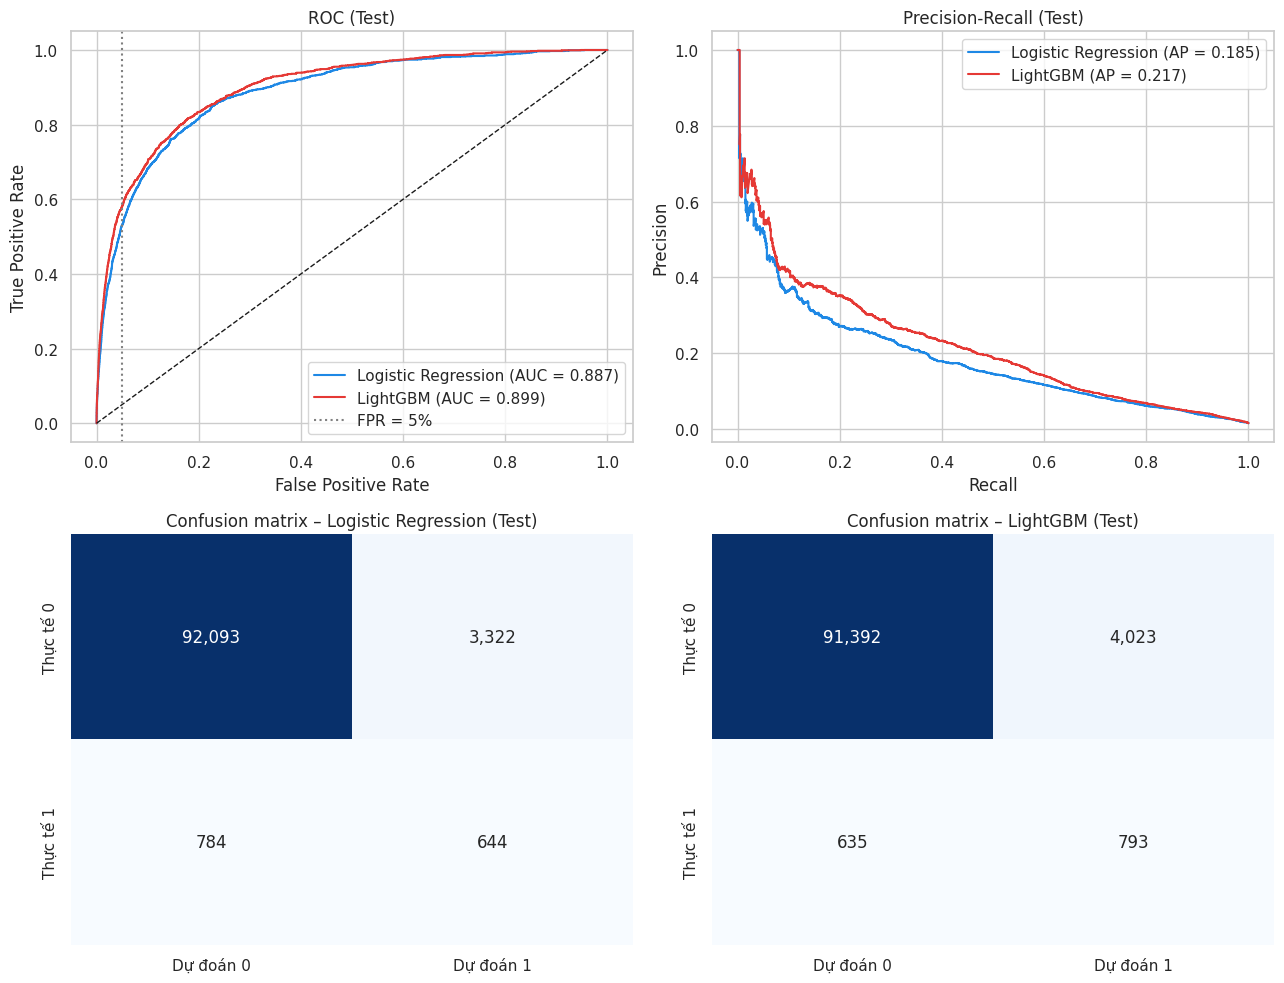
\includegraphics[width=0.90\linewidth]{tabular/c84_f0.png}
  \caption{Đường cong ROC, Precision-Recall và ma trận nhầm lẫn của Logistic Regression và LightGBM trên tập Test (tháng 7).}
  \label{fig:tab_roc_cm}
\end{figure}

\subsubsection{Đóng góp đặc trưng và độ hiệu chỉnh xác suất}
Phân tích mức độ đóng góp đặc trưng theo chỉ số \textit{Gain} trung bình qua 3 seed của LightGBM (\Cref{fig:tab_feat_imp}) cho thấy nhiều đặc trưng thiết kế trực tiếp từ giả thuyết EDA — như \texttt{limit\_per\_income}, \texttt{addr\_per\_age}, \texttt{bank\_per\_age} và cờ \texttt{prev\_address\_months\_count\_flag} — đều nằm trong nhóm 15 biến quan trọng nhất. Về độ hiệu chỉnh xác suất (\textit{Calibration}), LightGBM không điều chỉnh trọng số lớp nên bảo toàn xác suất tiên nghiệm, đạt \textit{Brier Score} trên Test bằng \textbf{0,01283} (có thể dùng trực tiếp để ước lượng tổn thất kỳ vọng); trái lại, Logistic Regression với \texttt{class\_weight='balanced'} làm xác suất đầu ra bị khuếch đại (\textit{Brier Score} = 0,09944), chỉ phù hợp cho mục đích xếp hạng.

\begin{figure}[H]
  \centering
  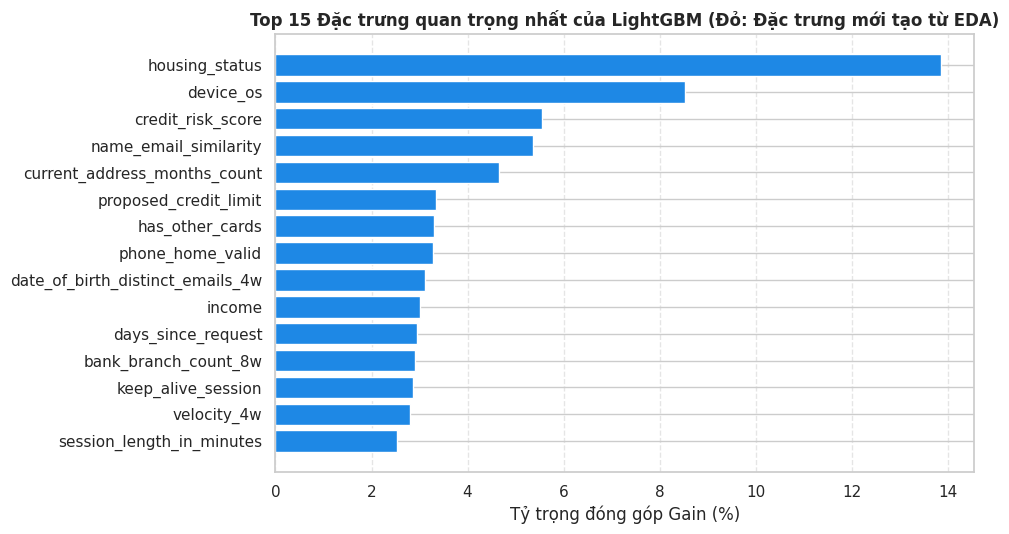
\includegraphics[width=0.84\linewidth]{tabular/c87_f0.png}
  \caption{Top 15 đặc trưng có tỷ trọng đóng góp \textit{Gain} lớn nhất trong LightGBM (màu đỏ đánh dấu các đặc trưng mới tạo từ phân tích EDA).}
  \label{fig:tab_feat_imp}
\end{figure}

\subsubsection{Đánh giá công bằng theo nhóm tuổi và đánh đổi vận hành}
Khi áp dụng ngưỡng chung 0,0478 của LightGBM trên tập Test (\Cref{fig:tab_fairness_policy}), tỷ lệ báo động nhầm của nhóm $\ge 50$ tuổi (12.667 hồ sơ) lên tới \textbf{10,12\%}, gấp ba lần nhóm $< 50$ tuổi (3,35\% trên 84.176 hồ sơ), kéo chỉ số $\text{FPR ratio} = \text{FPR}(<50)/\text{FPR}(\ge 50)$ xuống còn \textbf{0,331}. Việc áp ngưỡng riêng cho từng nhóm trên Validation đưa tỷ lệ báo động nhầm về trạng thái cân bằng (4,63\% so với 4,56\%, $\text{FPR ratio} = \mathbf{1,014}$), nhưng kéo theo sự sụt giảm rõ rệt về khả năng phát hiện gian lận ở nhóm $\ge 50$ tuổi (TPR giảm từ 71,29\% xuống 52,63\%, TPR toàn cục giảm từ 55,53\% xuống 54,20\%).

Hai thực nghiệm phụ được thực hiện để làm rõ cơ chế thiên lệch. Thứ nhất, khi loại bỏ hoàn toàn \texttt{customer\_age} và hai biến tỷ lệ chứa tuổi (\textit{Fairness through Unawareness}), FPR nhóm $\ge 50$ tuổi vẫn giữ ở mức 8,68\% so với 3,68\% của nhóm trẻ ($\text{FPR ratio} = 0,425$). Một mô hình phụ huấn luyện trên các biến còn lại vẫn dự đoán được nhóm tuổi $\ge 50$ với \textbf{AUC = 0,835}, chứng tỏ thông tin tuổi bị rò rỉ mạnh qua các biến gián tiếp (\textit{proxy leakage}), bên cạnh chênh lệch tỷ lệ gian lận nền vốn có. Thứ hai, khảo sát điểm đánh đổi trung gian với mục tiêu FPR 6,5\% trên Validation cho nhóm $\ge 50$ tuổi đạt FPR thực tế 6,01\% và giữ được TPR 59,33\% trên Test. Trong thực tiễn, thay vì tự động từ chối hồ sơ bằng ngưỡng phân biệt theo tuổi (có thể vướng quy định pháp lý), hướng tiếp cận phù hợp hơn là chuyển các hồ sơ bị cảnh báo sang bước xác thực bổ sung hoặc duyệt thủ công kết hợp giám sát FPR/TPR định kỳ theo nhóm nhân khẩu học.

\begin{figure}[H]
  \centering
  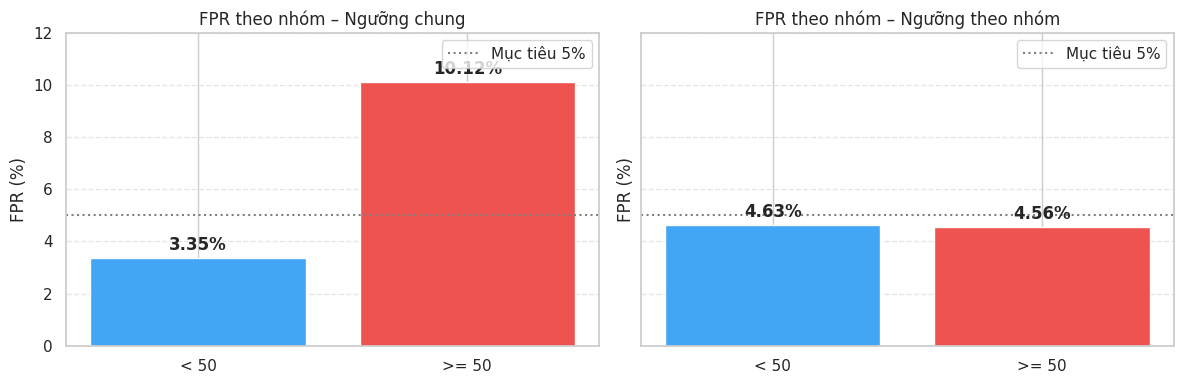
\includegraphics[width=0.86\linewidth]{tabular/c90_f0.png}
  \caption{So sánh tỷ lệ báo động nhầm (FPR) giữa hai nhóm tuổi dưới chính sách ngưỡng chung ($\text{FPR ratio} = 0,331$) và ngưỡng riêng theo nhóm ($\text{FPR ratio} = 1,014$).}
  \label{fig:tab_fairness_policy}
\end{figure}

\subsubsection{Kiểm chứng thực nghiệm giả thuyết EDA và phương pháp chia tập}
Hai thực nghiệm đối chứng cuối cùng trên cả Logistic Regression và LightGBM (\Cref{fig:tab_ablations}) xác nhận hai quyết định thiết kế nền tảng của bài toán:
\begin{enumerate}[leftmargin=*]
  \item \textbf{Tác động của 6 cột khuyết và 6 cờ \texttt{\_flag}:} Khi loại bỏ hoàn toàn nhóm đặc trưng này (còn 27 biến), \texttt{TPR@FPR5\%} giảm từ 0,5301 xuống 0,5035 ở Logistic Regression và từ 0,5798 xuống 0,5448 ở LightGBM (\texttt{ROC-AUC} giảm từ 0,8986 xuống 0,8837). Đáng chú ý, nếu chỉ bỏ 6 cờ \texttt{\_flag} và giữ 6 cột gốc, Logistic Regression sụt giảm ngay (0,5301 $\rightarrow$ 0,5056) vì phép điền trung vị xóa mất dấu hiệu MNAR, còn LightGBM gần như giữ nguyên (0,5749) nhờ cơ chế rẽ nhánh mặc định cho \texttt{NaN}. Kết hợp giữ \texttt{NaN} và 6 cờ \texttt{\_flag} vì thế mang lại lợi ích nhất quán cho cả hai họ mô hình.
  \item \textbf{Temporal Split so với Stratified Random Split:} Chia ngẫu nhiên 80/10/10 trộn lẫn cả 8 tháng tạo ra độ lạc quan giả tạo khi đánh giá (ngay cả khi lọc riêng lát cắt tháng 7 trong tập Test ngẫu nhiên, \texttt{TPR@ngưỡng} của Logistic Regression bị đẩy từ 0,4510 lên 0,4915 và của LightGBM lên 0,5763). Quan trọng hơn, ngưỡng chọn từ tập Validation trộn lẫn không phản ánh sự dịch chuyển của tháng 7, khiến FPR của LightGBM trên lát cắt tháng 7 tăng vọt lên \textbf{6,34\%}, phá vỡ ngân sách $\le 5\%$.
\end{enumerate}

\begin{figure}[H]
  \centering
  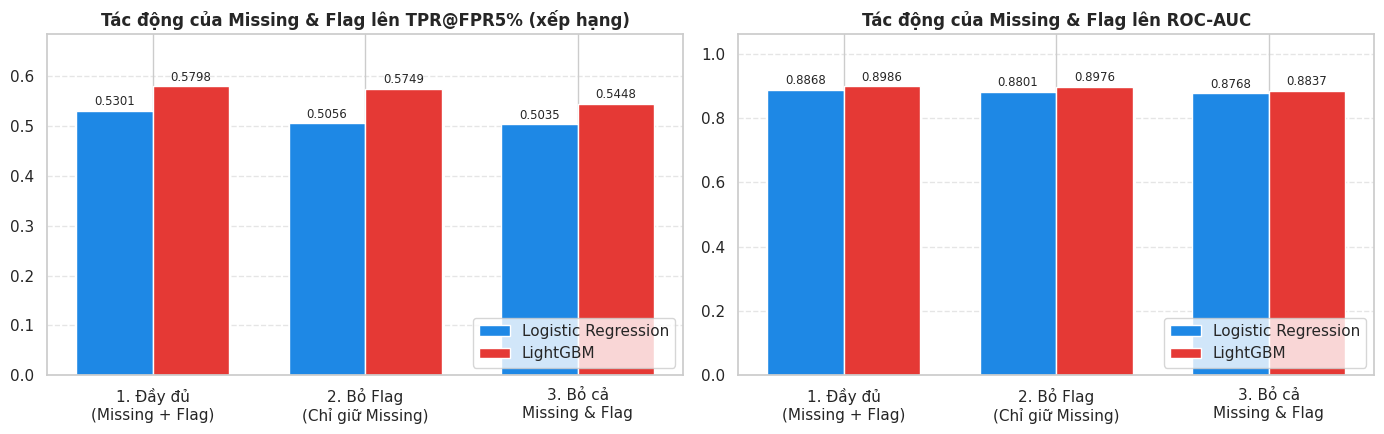
\includegraphics[width=0.90\linewidth]{tabular/c96_f0.png}\\[4pt]
  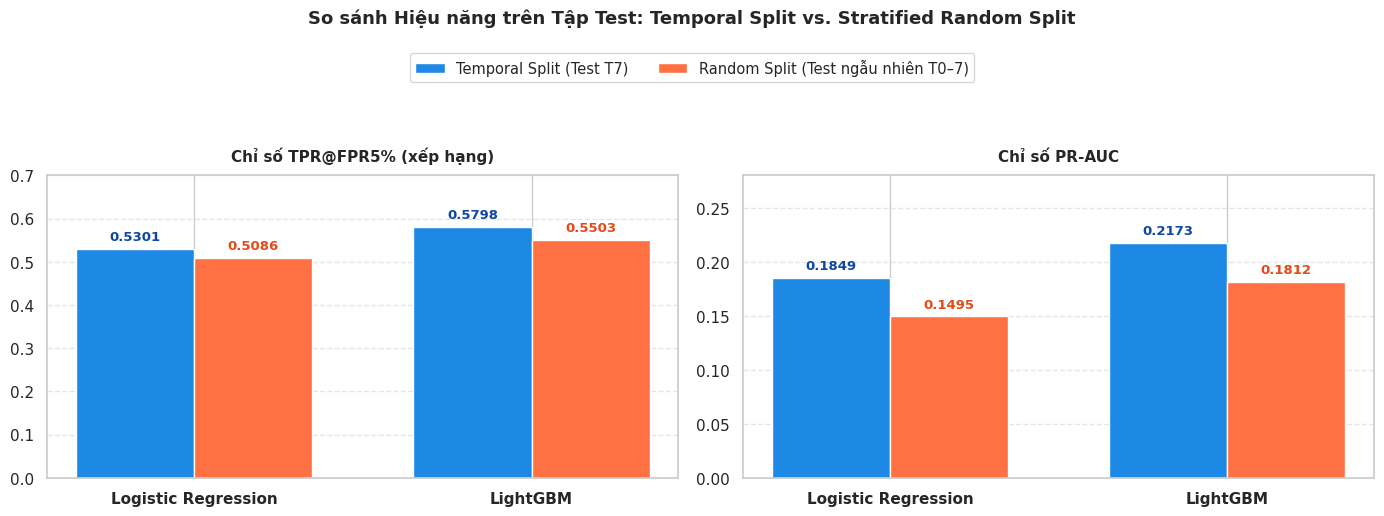
\includegraphics[width=0.90\linewidth]{tabular/c99_f0.png}
  \caption{Hai thực nghiệm kiểm chứng trên tập Test: tác động khi loại bỏ cột khuyết và cờ \texttt{\_flag} (trên) và so sánh \textit{Temporal Split} với \textit{Stratified Random Split} (dưới).}
  \label{fig:tab_ablations}
\end{figure}
